% Version 1.2 of SN LaTeX, November 2022
%
% See section 11 of the User Manual for version history 
%
%%%%%%%%%%%%%%%%%%%%%%%%%%%%%%%%%%%%%%%%%%%%%%%%%%%%%%%%%%%%%%%%%%%%%%
%%                                                                 %%
%% Please do not use \input{...} to include other tex files.       %%
%% Submit your LaTeX manuscript as one .tex document.              %%
%%                                                                 %%
%% All additional figures and files should be attached             %%
%% separately and not embedded in the \TeX\ document itself.       %%
%%                                                                 %%
%%%%%%%%%%%%%%%%%%%%%%%%%%%%%%%%%%%%%%%%%%%%%%%%%%%%%%%%%%%%%%%%%%%%%

%%\documentclass[referee,sn-basic]{sn-jnl}% referee option is meant for double line spacing

%%=======================================================%%
%% to print line numbers in the margin use lineno option %%
%%=======================================================%%

%%\documentclass[lineno,sn-basic]{sn-jnl}% Basic Springer Nature Reference Style/Chemistry Reference Style

%%======================================================%%
%% to compile with pdflatex/xelatex use pdflatex option %%
%%======================================================%%

%%\documentclass[pdflatex,sn-basic]{sn-jnl}% Basic Springer Nature Reference Style/Chemistry Reference Style


%%Note: the following reference styles support Namedate and Numbered referencing. By default the style follows the most common style. To switch between the options you can add or remove “Numbered” in the optional parenthesis. 
%%The option is available for: sn-basic.bst, sn-vancouver.bst, sn-chicago.bst, sn-mathphys.bst. %  
 
%%\documentclass[sn-nature]{sn-jnl}% Style for submissions to Nature Portfolio journals
%%\documentclass[sn-basic]{sn-jnl}% Basic Springer Nature Reference Style/Chemistry Reference Style
\documentclass[sn-mathphys,Numbered]{sn-jnl}% Math and Physical Sciences Reference Style
%%\documentclass[sn-aps]{sn-jnl}% American Physical Society (APS) Reference Style
%%\documentclass[sn-vancouver,Numbered]{sn-jnl}% Vancouver Reference Style
%%\documentclass[sn-apa]{sn-jnl}% APA Reference Style 
%%\documentclass[sn-chicago]{sn-jnl}% Chicago-based Humanities Reference Style
%%\documentclass[default]{sn-jnl}% Default
%%\documentclass[default,iicol]{sn-jnl}% Default with double column layout

%%%% Standard Packages
%%<additional latex packages if required can be included here>

\usepackage{graphicx}%
\usepackage{multirow}%
\usepackage{amsmath,amssymb,amsfonts}%
\usepackage{amsthm}%
\usepackage{mathrsfs}%
\usepackage[title]{appendix}%
\usepackage{xcolor}%
\usepackage{textcomp}%
\usepackage{manyfoot}%
\usepackage{booktabs}%
\usepackage{algorithm}%
\usepackage{algorithmicx}%
\usepackage{algpseudocode}%
\usepackage{listings}%
%%%%

%%%%%=============================================================================%%%%
%%%%  Remarks: This template is provided to aid authors with the preparation
%%%%  of original research articles intended for submission to journals published 
%%%%  by Springer Nature. The guidance has been prepared in partnership with 
%%%%  production teams to conform to Springer Nature technical requirements. 
%%%%  Editorial and presentation requirements differ among journal portfolios and 
%%%%  research disciplines. You may find sections in this template are irrelevant 
%%%%  to your work and are empowered to omit any such section if allowed by the 
%%%%  journal you intend to submit to. The submission guidelines and policies 
%%%%  of the journal take precedence. A detailed User Manual is available in the 
%%%%  template package for technical guidance.
%%%%%=============================================================================%%%%

%\jyear{2021}%

%% as per the requirement new theorem styles can be included as shown below
\theoremstyle{thmstyleone}%
\newtheorem{theorem}{Theorem}%  meant for continuous numbers
%%\newtheorem{theorem}{Theorem}[section]% meant for sectionwise numbers
%% optional argument [theorem] produces theorem numbering sequence instead of independent numbers for Proposition
\newtheorem{proposition}[theorem]{Proposition}% 
%%\newtheorem{proposition}{Proposition}% to get separate numbers for theorem and proposition etc.

\theoremstyle{thmstyletwo}%
\newtheorem{example}{Example}%
\newtheorem{remark}{Remark}%

\theoremstyle{thmstylethree}%
\newtheorem{definition}{Definition}%

\raggedbottom
%%\unnumbered% uncomment this for unnumbered level heads

\begin{document}

\title[An Effectively Complexity-reduced Language Model for Text Classification]{DistilBERT: An Effectively Complexity-reduced Language Model for Text Classification}

%%=============================================================%%
%% Prefix	-> \pfx{Dr}
%% GivenName	-> \fnm{Joergen W.}
%% Particle	-> \spfx{van der} -> surname prefix
%% FamilyName	-> \sur{Ploeg}
%% Suffix	-> \sfx{IV}
%% NatureName	-> \tanm{Poet Laureate} -> Title after name
%% Degrees	-> \dgr{MSc, PhD}
%% \author*[1,2]{\pfx{Dr} \fnm{Joergen W.} \spfx{van der} \sur{Ploeg} \sfx{IV} \tanm{Poet Laureate} 
%%                 \dgr{MSc, PhD}}\email{iauthor@gmail.com}
%%=============================================================%%

\author*[1,3,4]{\fnm{Ngoc-Thien-An} \sur{Pham}}\email{pntan19@clc.fitus.edu.vn}

\author[2,3,4]{\fnm{Hoang-Quan} \sur{Tran}}\email{19120338@student.hcmus.edu.vn}
\equalcont{These authors contributed equally to this work.}

% \author[1,2]{\fnm{Third} \sur{Author}}\email{iiiauthor@gmail.com}
% \equalcont{These authors contributed equally to this work.}

\affil*[1]{\orgdiv{Department of Computer Science}}

\affil[2]{\orgdiv{Department of Knowledge Engineering}}

\affil[3]{\orgname{Faculty of Information Technology, University of Science}}

\affil[4]{\orgname{Vietnam National University}, \orgaddress{\city{Ho Chi Minh City}, \country{Vietnam}}}


%%==================================%%
%% sample for unstructured abstract %%
%%==================================%%

\abstract{Text classification has been a fundamental task dating back to the early days of Natural Language Processing and has received increased attention in recent academic literature. This task is the process of categorizing text documents into predefined classes or categories based on their content. Currently, the invention of large language models such as BERT, RoBERTa, XLM, and others has started a revolution in Natural Language Processing, specifically in Text Classification and text-related tasks. However, these models require an enormous textual dataset, a high-cost training environment, and a long training time to achieve a notable result. This paper presents a novel approach to Text Classification using a lighter, cheaper, faster version of BERT called DistilBERT. By fine-tuning DistilBERT for the Text Classification task, we achieved a state-of-the-art result of 97.40\%, 97.61\%, 97.74\%, and 97.64\% in accuracy, macro precision, macro recall, and macro F1 respectively. With these evaluation scores, our model achieves the comparable results to the current state-of-the-art language model's in the text classification task.}

%%================================%%
%% Sample for structured abstract %%
%%================================%%

% \abstract{\textbf{Purpose:} The abstract serves both as a general introduction to the topic and as a brief, non-technical summary of the main results and their implications. The abstract must not include subheadings (unless expressly permitted in the journal's Instructions to Authors), equations or citations. As a guide the abstract should not exceed 200 words. Most journals do not set a hard limit however authors are advised to check the author instructions for the journal they are submitting to.
% 
% \textbf{Methods:} The abstract serves both as a general introduction to the topic and as a brief, non-technical summary of the main results and their implications. The abstract must not include subheadings (unless expressly permitted in the journal's Instructions to Authors), equations or citations. As a guide the abstract should not exceed 200 words. Most journals do not set a hard limit however authors are advised to check the author instructions for the journal they are submitting to.
% 
% \textbf{Results:} The abstract serves both as a general introduction to the topic and as a brief, non-technical summary of the main results and their implications. The abstract must not include subheadings (unless expressly permitted in the journal's Instructions to Authors), equations or citations. As a guide the abstract should not exceed 200 words. Most journals do not set a hard limit however authors are advised to check the author instructions for the journal they are submitting to.
% 
% \textbf{Conclusion:} The abstract serves both as a general introduction to the topic and as a brief, non-technical summary of the main results and their implications. The abstract must not include subheadings (unless expressly permitted in the journal's Instructions to Authors), equations or citations. As a guide the abstract should not exceed 200 words. Most journals do not set a hard limit however authors are advised to check the author instructions for the journal they are submitting to.}

\keywords{Text classification, Natural language processing, Deep learning, Knowledge distillation, Pretrained language models}

%%\pacs[JEL Classification]{D8, H51}

%%\pacs[MSC Classification]{35A01, 65L10, 65L12, 65L20, 65L70}

\maketitle


\section{Introduction}\label{introduction}
Text classification constitutes a crucial problem in the field of natural language processing (NLP). Its significance lies in its diverse range of applications, including but not limited to document organization, news filtering, spam detection, opinion mining, and computational phenotyping\cite{Aggarwal2012, Zeng2019}. Text representation plays a vital role in text classification, as it converts raw textual data into a format that can be efficiently processed by machine learning algorithms. 

Traditionally, text was represented using hand-crafted features such as sparse lexical features, for instance, bag-of-words and $n$-grams. However, recent advances in deep learning have resulted in the widespread use of convolutional neural networks (CNN)\cite{LeCun1998}, recurrent neural networks (RNN)\cite{Rumelhart1987}, and long short-term memory (LSTM)\cite{Hochreiter1997}, to learn text representations automatically. According to a recent paper by Gasparetto et al. (2022)\cite{Gasparetto2022}, using pre-trained language models such as BERT\cite{Devlin2019} and RoBERTa\cite{Liu2019} can significantly improve text representation and enhance text classification performance. They reported state-of-the-art results on various benchmark datasets, demonstrating the superiority of deep learning-based methods over traditional feature-based approaches.

Although autoencoding-based pre-trained models such as BERT or RoBERTa embrace the capacity of modelling directional context at scale, the size of these models presents a noticeable challenge. Because their depth necessitates a large number of parameters that must be loaded into memory. This is not solely limited to the training phase and may pose challenges in real-world scenarios, particularly when pre-trained models are employed for inference under low-latency constraints or fine-tuning in settings with limited resources. In order to overcome this challenge, various strategies have been devised to create more compact models with fewer parameters. One successful approach to achieve this objective is through knowledge distillation. 

In this paper, based on these observations, we innovatively propose an approach to the Text Classification problem by adapting a distilled version of BERT, which is called DistilBERT\cite{Sanh2019}. To the best of our knowledge, we are the first to adapt DistilBERT to solve the Text Classification problem. Our proposal shows its nearly equivalent performance as BERT while considerably reducing the number of parameters. Our code is available at: \href{https://github.com/trhgquan/MNC}{https://github.com/trhgquan/MNC}

The trained weights, in conjunction with the training code available in the Transformers library from HuggingFace (Wolf et al., 2019)\cite{Wolf2019}, have been employed to facilitate the fine-tuning process on domain-specific datasets.

\paragraph{Contribution}
Our contributions are summarized as follows:
We propose a knowledge distillation-based method for text classification. 
\begin{itemize}
    \item Our proposal can be more appropriate for real-world appliances by its viability of inferencing under low-latency constraints or well-functioning in limited computational resources.
    \item Our experimental results demonstrate that the proposal achieves comparable performance against those attained by state-of-the-art text classification methods on several benchmark datasets.
\end{itemize}

\paragraph{Organization}
We structure the paper into 5 sections. In Section~\ref{introduction}, the context of Text Classification is introduced and the motivation we draw to improve the performance of this problem. Next, we investigate some proposals published in recent literature in Section~\ref{relatedworks} before providing our models in detail in Section~\ref{proposedmethod}. After that, we analyze some aspects of our model in Section~\ref{experiments} prior to including some directions for future research in Section~\ref{conclusionandfutureworks}.


\section{Related works}\label{relatedworks}
In the context of Text Classification, methods are divided into two main taxonomies, including shallow and deep learning approaches. Shallow learning approaches have replaced rule-based methods in terms of accuracy and stability. While still popular in many practical contexts, these methods have limitations in processing large amounts of data. They are particularly useful when resources for deep methods are limited but require costly feature engineering, which can be challenging depending on the complexity of the domain. While deep learning models have become popular due to their capacity to extract complex features without the need for hand-engineering, thereby reducing the domain knowledge requirement. Instead, efforts have been directed towards developing neural network architectures capable of extracting effective textual representations. Recent advancements have been particularly fruitful in this regard, generating semantically meaningful and contextual representations. Automated feature extraction is particularly advantageous in modelling textual data, as it can leverage the inherent linguistic structure of a document. While the linguistic structure of a document may be intuitive to humans, it is often incomprehensible to machines.

\subsection{Shallow machine-learning models}

Early approach to the Text Classification problem using rule-based systems where an expert suggests a rule for classifying text, based on the semantics and pragmatics of the data. Later on, several methods including Naive Bayes\cite{Xu2017}, Decision Trees\cite{Safavian1991}, Logistic Regression\cite{Genkin2007} and Support Vector Machine (SVM)\cite{boser1992, cortesvapnik1995} were proposed with the concept of using the probability of tokens to predict if a document belongs to a specific class. 

These approaches are easy to implement and perform best with a small amount of data. Besides advantages, shallow models have some disadvantages by requiring a feature engineering step to be effective. Additionally, shallow learning models are depending on the probability of each token, which is not capturing the general semantics of a complex document.

\subsection{Deep learning models}
Deep learning approaches, on the other hand, learn features automatically from the data, eliminating the need for extensive feature engineering. These methods include Convolutional Neural Networks (CNN)\cite{Kim2014}, Recurrent Neural Networks (RNN)\cite{Sutskever2014}, combinations between CNN and RNN\cite{Vo2017}, and Transformer-based models (BERT, XLM)\cite{Devlin2019, Conneau2020}. These models have shown state-of-the-art performance on many text classification tasks but require significantly more computational resources and data to train effectively. However, these models are highly scalable, making them suitable for processing large amounts of text data.

Our research is motivated by the application of knowledge distillation-based networks\cite{Gasparetto2022} in Text Classification, as previously explored in the literature. But we further investigate several perspectives of our proposal, including its compatibility, complexity, and efficiency.

\section{Proposed method}\label{proposedmethod}
In our proposed model, the initialization of representations for tokens is achieved by using a BERT-style model (e.g, BERT, RoBERTa, or DistilBERT). DistilBERT generates token embeddings through a process known as contextualized embedding as BERT does. Specifically, the model utilizes pre-trained neural networks that have been trained on large corpora to generate context-aware word embeddings for text representations. These representations are used as inputs to DistilBERT.

Next, the outputs of DistilBERT model are a sequence of token embeddings. Subsequently, the output token \texttt{[CLS]} is fed into a final fully-connected layer with parameters $W \in \mathbb{R}^{D\times H}$ and $b \in \mathbb{R}^H$. In that, $D$ is the dimensionality of the output vector and H denotes the number of classes needed for classifying. Finally, to predict the label, the softmax layer is applied to the new projected vector. During fine-tuning, the cross-entropy and binary cross-entropy loss functions are employed for the minimization process in single-label and multi-label tasks, respectively. The overall framework of our model is depicted in the Figure~\ref{fig:distilbert}. Depending on each type of dataset, these loss functions are based on the comparison between the predicted probability distribution and the actual label distribution, with the objective of minimizing the discrepancy between them.

\begin{figure}[htp]
\centering
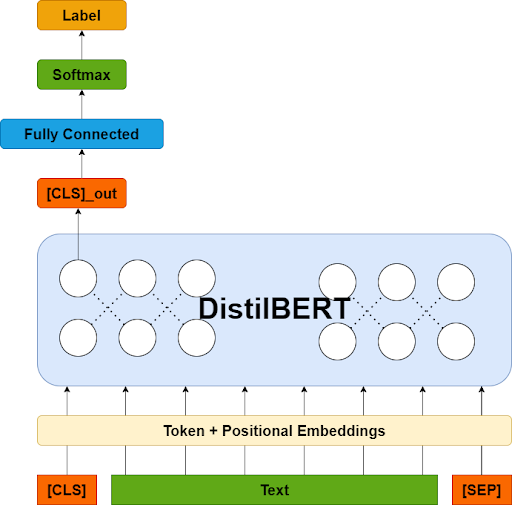
\includegraphics[scale=.4]{distilbert.png}
\caption{The overall architecture of our proposed method using DistilBERT.}
\label{fig:distilbert}
\end{figure}

\section{Experiments}\label{experiments}
\subsection{Baselines}
We compare our proposed model against multiple state-of-the-art text classification methods:
\begin{itemize}
\item \textbf{Shallow models}: Shallow text classification models include Logistic Regression, Naive Bayes, and Support Vector Machine. In contrast to deep learning methods, these models do not require a significant amount of training data to achieve a comparable result.
\item \textbf{CNN}: The Convolutional Neural Network (CNN) approach was introduced by Kim et al (2014)\cite{Kim2014}. Using an unsupervised learning model, an input word is converted into a word representation vector in a contextual space. These vectors are then stacked together to form a sentence-representation matrix. Finally, using a simple CNN with one layer of convolution on top of pre-trained word vectors.
\item \textbf{RNN and Sequence-to-Sequence}: Sutskever et al. (2014)\cite{Sutskever2014} proposed an architecture named Sequence-to-Sequence (Seq2Seq) to solve the Machine Translation problem, then used in Text Classification. In our experiments, we use Bidirectional Gated Recurrent Unit (BiGRU)\cite{Cho2014-GRU} instead of RNN blocks in the original work to fasten the training progress while ensuring the information is well-captured in both directions with Bidirectional architecture.
\item \textbf{CNN + LSTM}: A combination of two previous well-known approaches was introduced by Vo et al. (2017)\cite{Vo2017} for Vietnamese Text Classification. An input sentence is fed into two different architectures including a CNN with different filter sizes and an LSTM Sequence-to-Sequence Encoder. The output vector of CNN is then concatenated with the hidden state output of the LSTM network to form a combination context vector, which would go through a fully connected layer to get the final probability distribution over classes. We implemented the original architecture by Vo et al (2017) and an improved version using BiGRU.
\item \textbf{BERT}: Vaswani et al. (2017)\cite{Vaswani2017} introduced Transformer as an effective architecture for Machine Translation and can be applied to various downstream tasks. Some advantages of Transformer compared to Sequence-to-Sequence models include capturing essential information, eliminating recurrent connection, and supporting parallel computing. The Encoder of Transformer is then used to create an independent language model called Bidirectional Encoder Representations from Transformers (BERT)\cite{Devlin2019}.
\item \textbf{XLM}: Conneau et al. (2020)\cite{Conneau2020} discovered that pretraining multilingual language models at scale leads to significant performance gains for a wide range of cross-lingual transfer tasks. As a result, XLM is introduced (trained on 100 languages with more than 2TB of filtered CommonCrawl data) which shows very strong benchmark results compared to monolingual models.
\end{itemize}

\subsection{Dataset}
We conduct experiments on 2 datasets: the TREC and the SST2 dataset. The details of each dataset will be present in following subsections:

\subsubsection{The TREC dataset}
The TREC dataset\cite{hovy2001, li2002} has 6 coarse labels and includes 6000 sentences divided into training/testing sets with 5500 sentences for training and 500 sentences for testing. We use the TREC training subset for training and finetuning while evaluations were made on the testing subset. The dataset’s statistics are briefly described in Table~\ref{tab:trec-insight}

\begin{table}[htp]
\centering
\caption{Insight of the TREC dataset} \label{tab:trec-insight}
\begin{tabular*}{\textwidth}{@{\extracolsep\fill}cccccc}
\toprule
\textbf{Training} & \textbf{Testing} & \textbf{Coarse labels} & \textbf{Fine class labels} & \textbf{Avg. length} & \textbf{Vocab. size} \\ \midrule
5500              & 500              & 6                      & 50                         & 10                   & 8700                 \\ \bottomrule
\end{tabular*}
\end{table}

\subsubsection{The SST2 dataset}
The SST2 dataset\cite{Socher2013} is a binary-class dataset made from 70042 sentences, divided into 3 training, validation, and testing subsets. The original testing set, however, is unlabeled, so we divide the training set into a ratio of 7:3 for training and validation and use the original validation set for testing. The SST2 dataset’s insights are described in Table~\ref{tab:sst2-insight}

\begin{table}[htp]
\centering
\caption{Insight of the SST2 dataset} \label{tab:sst2-insight}
\begin{tabular*}{\textwidth}{@{\extracolsep\fill}cccc}
\toprule
\textbf{Training} & \textbf{Validation} & \textbf{Testing} & \textbf{Labels} \\ \midrule
47144              & 20205              & 872                      & 2 \\ \bottomrule
\end{tabular*}
\end{table}


\subsection{Experimental Setup}
\subsubsection{Training strategy}
\paragraph{Shallow models}
We build a data pipeline using \texttt{sklearn} (Pedregosa et al., 2011)\cite{Pedregosa2011} CountVectorizer with the $n$-grams range of 1 and 2; combined with TfidfTransformer with inverse-document-frequency reweighting enabled. The classifiers used in the experiments are Logistic Regression with L2 penalty, Naive Bayes, and Support Vector Classifier.

\paragraph{BiGRU Seq2Seq} 
Based on the architecture proposed by Sutskever et al. (2014), we replicated a Seq2Seq architecture with random embedding size of 256, 4 BiGRU layers with a hidden size of 512, and a dropout rate of 0.5. Training is set to 1000 epochs with early stopping after 20 epochs, batch size of 64, and learning rate of 0.001. The optimizer is Adam, with a learning rate decay step size of 1 and multiplicative factor of 0.1

\paragraph{CNN} 
Following Kim et al. (2014), we use filter sizes of 2, 3, and 4 with 2 filters each. The dropout rate is set at 0.5 while the learning rate is set at 0.25. In most CNN experiments, the optimizer used is AdaDelta with the \texttt{rho} coefficient set at 0.95. 

We applied a method called fastText (Joulin et al., 2017)\cite{Joulin2017} designed for word representation to improve the original architecture by speeding up training progress while also improving training metrics. The embedding size in this scenario is fixed by fastText, while in the original architecture with random embedding, the dimension is fixed at 300. We trained 3 versions using random embeddings, non-trainable fastText embedding, and a trainable fastText embedding in 20 epochs under the same random seed.

\paragraph{Multi-channel CNN with RNN}
We employ the multi-channel CNN with LSTM architecture by Vo et al. (2017). The filter sizes is set to 3, 4, and 5 with 150 filters each. We use the random embedding dimension of 200, and the LSTM hidden dimension of 100 with 128 hidden units. We set the dropout rate at 0.2, and the learning rate at 0.25 for 50 epochs of training under the same random seed.

With the improved version, we replace LSTM with 128 hidden units BiGRU blocks and replacing the random embedding layer with a fastText embedding layer. The filter size is then updated to 3, 5, and 7 while the number of filters is set at 150. The learning rate in this scenario is 1, set for 50 epochs of training.

\subsubsection{Finetuning strategy}
To finetune BERT, we use \texttt{bert-base-uncased}\footnote{\url{https://huggingface.co/bert-base-uncased}} from Huggingface (originally has 110 millions parameters, trained on English corpora) as the pre-train model. With the finetuning strategy, we set the learning rate to 2e-5, the weight decay to 0.01, and the batch size to 16 while the number of training epochs are different on different datasets:
\begin{itemize}
\item On  the TREC dataset, we finetune BERT in 10 epochs with early stopping patience set to 3 epochs.
\item On the SST2 dataset, due to the limitations of training hardware we set the training progress to stop after 1 epoch.
\end{itemize}

The finetuning of XLM-RoBERTa and DistilBERT use \texttt{xlm-roberta-base}\footnote{\url{https://huggingface.co/xlm-roberta-base}} and \texttt{distilbert-base-uncased}\footnote{\url{https://huggingface.co/distilbert-base-uncased}} from Huggingface as pre-train models, respectively. We use the same finetuning strategy with BERT to finetune XLM-RoBERTa and DistilBERT on TREC and SST2 datasets.

\subsubsection{Evaluation Metrics}
We use Accuracy, Macro Precision, Macro Recall and Macro F1 Score as evaluation metrics. The definition of each metric is presented in the following sections.

\paragraph{Accuracy}
Assuming the testing set has $n$ samples, let $\hat{y}_i$ and $y_i$ be the $i$-th sentence predicted label and ground-truth label respectively. Hence, the Accuracy metric will be defined as total correctly predicted labels divided by total labels, defined in Equation~\ref{eq:accuracy}.

\begin{equation}\label{eq:accuracy}
\text{Accuracy} = \frac{1}{n}\displaystyle\sum_{i = 1}^n (y_i = \hat{y_i})
\end{equation}

\paragraph{Precision, Recall and F1 Score}
Given a class $C$, let $TP$ be the total correctly-labelled samples of class $C$ (\textit{true positive} samples); $FP$ be the total samples not belonging to but incorrectly labelled as $C$ (\textit{false positive} samples), and $FN$ be the total samples belonging to $C$ but incorrectly labelled as another class (\textit{false negative} samples). Hence, the Precision metric would be defined as Equation~\ref{eq:precision}
\begin{equation}\label{eq:precision}
\text{Precision (P)} = \frac{TP}{TP + FP}    
\end{equation}
the Recall metric would be defined as Equation~\ref{eq:recall}
\begin{equation}\label{eq:recall}
\text{Recall (R)} = \frac{TP}{TP + FN}
\end{equation}
and the F1 Score would be defined as Equation~\ref{eq:f1}
\begin{equation}\label{eq:f1}
\text{F1} = \frac{2PR}{P + R}
\end{equation}

\paragraph{Micro and Macro metrics}
Take an example of a classification problem with $n$ labels using Precision metric. With $TP_1, TP_2, .., TP_n$; $FP_1, FP_2, .., FP_n$ are total \textit{true positive} and \textit{false positive} samples of $n$ classes. The Micro Precision and Macro Precision metrics would be defined as Equation~\ref{eq:micro-macro-precision}

\begin{equation}\label{eq:micro-macro-precision}
\begin{aligned}
\text{Precision}_{micro} &= \frac{TP_1 + TP_2 + .. + TP_n}{(TP_1 + FP_1) + (TP_2 + FP_2) + .. + (TP_n + FP_n)} \\
&= \frac{\displaystyle\sum_{i = 1}^n TP_i}{\displaystyle\sum_{i = 1}^n (TP_i + FP_i)} \\
\text{Precision}_{macro} &= \frac{1}{n}\left[\left(\frac{TP_1}{TP_1 + FP_1}\right) + \left(\frac{TP_2}{TP_2 + FP_2}\right) + .. + \left(\frac{TP_n}{TP_n + FP_n}\right)\right] \\
&= \frac{1}{n}\sum_{i = 1}^n \frac{TP_i}{TP_i + FP_i}
\end{aligned}
\end{equation}

\subsubsection{Results}
We use the same initial random seeds for every experiment. To guarantee objectivity and fairness, we run our experiments five times. The results nearly remain the same. Table~\ref{tab:result} reports the Accuracy, Macro Precision, Macro Recall and Macro F1 of the baselines and the proposed method on both the TREC and SST2 testing sets.

\begin{sidewaystable}[htp]
\caption{Experiment metrics two benchmark datasets. Bold indicates the highest scores.} \label{tab:result}
\begin{tabular*}{\textwidth}{@{\extracolsep\fill}lcccccccc}
\toprule
& \multicolumn{4}{@{}c@{}}{\textbf{TREC}}& \multicolumn{4}{@{}c@{}}{\textbf{SST2}} \\\cmidrule{2-5}\cmidrule{6-9}%
\multicolumn{1}{c}{\textbf{Model}}                    & \multicolumn{1}{c}{\textbf{Accuracy}} & \multicolumn{1}{c}{\textbf{Precision}} & \multicolumn{1}{c}{\textbf{Recall}} & \multicolumn{1}{c}{\textbf{F1}} & \multicolumn{1}{c}{\textbf{Accuracy}} & \multicolumn{1}{c}{\textbf{Precision}} & \multicolumn{1}{c}{\textbf{Recall}} & \multicolumn{1}{c}{\textbf{F1}}\\ \midrule
Logistic Regression   & 0.852 & 0.831          & 0.897       & 0.856  & 0.807 & 0.806 & 0.810 & 0.807 \\
Multinomial Naive Bayes   & 0.832 & 0.704          & 0.699       & 0.697  & 0.808 & 0.807 & 0.819 & 0.806        \\
Support Vector Classifier & 0.886 & 0.862          & 0.912       & 0.882  & 0.829 & 0.829 & 0.830 & 0.829        \\ \midrule
BiGRU Seq2Seq            & 0.836 & 0.695          & 0.708       & 0.700   & 0.765 & 0.766 & 0.764 & 0.764       \\ \midrule
CNN + random embedding                 & 0.726 & 0.809          & 0.684       & 0.718   & 0.760 & 0.774 & 0.758& 0.756       \\
CNN + fastText (freeze)   & 0.924 & 0.933          & 0.898       & 0.912    & 0.830 & 0.834 & 0.829 & 0.830      \\
CNN + fastText (trainable) & 0.910 & 0.922          & 0.885       & 0.899   & 0.843 & 0.851 & 0.842 & 0.842       \\
\midrule
CNN + LSTM + random embedding  & 0.652 & 0.717          & 0.637       & 0.631  & 0.734 & 0.741 & 0.735 & 0.733 \\
CNN + BiGRU + random embedding     & 0.676 & 0.717          & 0.701       & 0.689  & 0.748 & 0.754 & 0.749 & 0.747 \\
CNN + BiGRU + fastText (freeze)   & 0.914 & 0.919          & 0.896       & 0.904   & 0.815 & 0.818 & 0.816 & 0.815 \\
CNN + BiGRU + fastText (trainable) & 0.902 & 0.892          & 0.884       & 0.886  & 0.806 & 0.813 & 0.805 & 0.805 \\ \midrule
Finetuned BERT & \textbf{0.976} & \textbf{0.978} & \textbf{0.982} & \textbf{0.979}  & 0.906 & 0.905 & 0.909 & 0.906 \\
Finetuned XLM-RoBERTa & 0.966 & 0.971          & 0.970       & 0.970  & \textbf{0.911} & \textbf{0.911} & \textbf{0.911} & \textbf{0.911} \\ \midrule
Finetuned DistilBERT\footnotemark[1]  & 0.974 & 0.976 & 0.977  & 0.976  & 0.905 & 0.904 & 0.906 & 0.905\\ \bottomrule
\end{tabular*}
\footnotetext[1]{Our proposed method}
\end{sidewaystable}

We also measured the inference time and total trainable parameters of deep approaches using the Google Colab environment. DistilBERT performs slower than CNN and Seq2Seq approaches with the same initial seed but is faster than approaches using LLMs. The inference time and total parameters of each model on the TREC and SST2 testing sets are presented in Table~\ref{tab:inference-result} and Table~\ref{tab:parameters-result}, respectively. 

\begin{table}[htp]
\caption{Inference time of deep learning approaches on testing sets}\label{tab:inference-result}
\begin{tabular*}{\textwidth}{@{\extracolsep\fill}lccc}
\toprule
 & \multicolumn{2}{@{}c@{}}{\textbf{Inference time\footnotemark[1]}} \\ \cmidrule{2-3}%
\textbf{Model}  & \textbf{TREC}  & \textbf{SST2}\\ \midrule
BiGRU Seq2Seq                      & 1.812 $\pm$ 0.668 ms &  3.394 $\pm$ 1.222 ms                     \\ \midrule
CNN + random embedding             & 1.673 $\pm$ 0.359 ms & 2.378 $\pm$ 0.747 ms                  \\
CNN + fastText (freeze)           & 1.610 $\pm$ 0.318 ms & 1.705 $\pm$ 0.379 ms                     \\
CNN + fastText (trainable)         & 1.658 $\pm$ 0.444 ms & 1.780 $\pm$ 0.329 ms                    \\ \midrule
CNN + LSTM + random embedding      & 5.626 $\pm$ 0.750 ms & 6.607 $\pm$ 1.010 ms                   \\
CNN + BiGRU + random embedding     & 11.387 $\pm$ 3.077 ms & 10.419 $\pm$ 1.635 ms                   \\
CNN + BiGRU + fastText (freeze)   & 10.211 $\pm$ 1.460 ms & 11.769 $\pm$ 3.032 ms                  \\
CNN + BiGRU + fastText (trainable) & 10.270 $\pm$ 2.187 ms & 13.386 $\pm$ 3.206 ms                  \\ \midrule
Finetuned BERT                     & 17.725 $\pm$ 4.071 ms & 16.984 $\pm$ 4.228 ms                  \\
Finetuned XLM-RoBERTa              & 16.933 $\pm$ 8.987 ms & 15.848 $\pm$ 3.840 ms                  \\ \midrule
Finetuned DistilBERT\footnotemark[2]               & 9.776 $\pm$ 2.499 ms & 9.629 $\pm$ 6.478 ms                    \\ \bottomrule
\end{tabular*}
\footnotetext[1]{Mean $\pm$ stdev}
\footnotetext[2]{Our proposed method}
\end{table}

\begin{table}[htp]
\caption{Total parameters of deep learning approaches}\label{tab:parameters-result}
\begin{tabular*}{\textwidth}{@{\extracolsep\fill}lccc}
\toprule
 & \multicolumn{2}{@{}c@{}}{\textbf{Total parameters}} \\ \cmidrule{2-3}%
\textbf{Model}  & \textbf{TREC}  & \textbf{SST2}\\ \midrule
BiGRU Seq2Seq                      & 18,461,702 &  20,254,722                     \\ \midrule
CNN + random embedding             & 3,192,606 & 4,802,702                  \\
CNN + fastText (freeze)           & 362,106 & 360,902                     \\
CNN + fastText (trainable)         & 3,192,606 & 4,802,702                    \\ \midrule
CNN + LSTM + random embedding      & 4,420,416 & 6,568,012                   \\
CNN + BiGRU + random embedding     & 4,504,896 & 6,652,492                   \\
CNN + BiGRU + fastText (freeze)   & 987,696 & 986,892                  \\
CNN + BiGRU + fastText (trainable) & 6,648,696 & 9,870,492                 \\ \midrule
Finetuned BERT                     & 108,314,886 & 108,311,810                  \\
Finetuned XLM-RoBERTa              & 278,048,262 & 278,045,186                  \\ \midrule
Finetuned DistilBERT\footnotemark[1]  & 65,786,118 & 65,783,042                    \\ \bottomrule
\end{tabular*}
\footnotetext[1]{Our proposed method}
\end{table}

\subsection{Analysis}
\subsubsection{Performance}
We evaluate the Accuracy, Macro Precision, Macro Recall and Macro F1 of shallow and deep approaches on the testing sets. This results are shown in Table~\ref{tab:result}. Deep approaches may require a longer training period in order to achieve a comparable result, while shallow approaches may be able to achieve a competitive result with minimal data. A notable insight is that using pre-trained sentence embedding such as fastText can boost metrics dramatically. With the CNN and CNN-ensemble architectures, replacing the random embedding layer with the fastText layer can boost metrics from 10\% to 20\%. Observations suggest that pre-trained sentence embeddings, such as fastText, are capable of capturing context and semantics from a sentence independently of the text classification model since they were trained on a large amount of data. Even though DistilBERT cannot achieve the best results when it comes to language models, it is close to the ideal result which has been achieved by BERT or XLM-RoBERTa. This is considered a comparable result, since DistilBERT theoretically has 40\% less parameters than BERT but preserves 95\% of BERT's performance.

\subsubsection{Inference time}
We evaluate the inference time of the deep learning models on the testing sets; the results are shown in Table \ref{tab:inference-result}. It can be seen that the inference times of the CNN based models and the BiGRU Seq2Seq model give the best results, being relatively fast at less than 2 ms. However, they compensate for the low accuracy when compared to DitilBERT. As for the models combining CNNs, the inference time is higher than our proposal, while fine-tuned BERT or XLM-RoBERTa have almost twice the inference time of DistilBERT. When it comes to accuracy, DistillBERT gives nearly the same results as these two language models, but the inference time is twice as fast (approximately 9.5 ms). Therefore, it is more feasible to use the distilled knowledge based model in practical applications in terms of both accuracy and low latency.

\subsubsection{Parameters}
Table \ref{tab:parameters-result} shows the total number of parameters of the machine learning models on the two aforementioned datasets. CNN-related models have significantly low numbers—less than 7 million parameters. Notably, the combined model of CNN and BiGRU with the frozen fastText embeddings had the smallest number of parameters compared to the other models. Surprisingly, the BiGRU Seq2Seq model has a significantly higher number of parameters when compared to the CNN models, with slightly under 18.5 million on the TREC and just over 20.25 million on the SST2, in contrast to the fast inference time in the above analysis. In terms of language models, DistilBERT has enormously fewer parameters than BERT (about 40 million parameters) and about four times fewer than XLM-RoBERTa.

\section{Conclusion and Future works}\label{conclusionandfutureworks}
In this work, we propose DistilBERT, a cheaper, lighter, and faster version of BERT, for Text Classification. Even though reducing the number of layers (e.g., attention heads), DistilBERT still shows its efficiency by the comparable achievements. Besides, we analyze deeper into related aspects of this knowledge distillation-based model, including performance, inference, and complexity. However, in this work, we only focus on investigating the architecture used without considering how to integrate more useful information (e.g., structural or hierarchical) which is crucial for the model to capture more meaningful contextual features. We leave this for future research.

%%===========================================================================================%%
%% If you are submitting to one of the Nature Portfolio journals, using the eJP submission   %%
%% system, please include the references within the manuscript file itself. You may do this  %%
%% by copying the reference list from your .bbl file, paste it into the main manuscript .tex %%
%% file, and delete the associated \verb+\bibliography+ commands.                            %%
%%===========================================================================================%%

\bibliography{sn-bibliography}% common bib file
%% if required, the content of .bbl file can be included here once bbl is generated
%%\input sn-article.bbl


\end{document}
